%%%%%%%%%%%%%%%%% Backup two slides

%% ------------------ ATTENUATION OF X-RAYS -----------------------
\frame{
\begin{tikzpicture}[remember picture,overlay]
\fill[blue1]
(current page.north west) rectangle ([xshift=0.33\paperwidth,yshift=0.33\paperheight]current page.west|-{pic cs:end});
\end{tikzpicture}

\begin{textblock}{0.5}(0.02,0.03)
	\textcolor{white}{
		\Large Attenuation of X-rays}
\end{textblock}

\begin{textblock}{0.45}(0.5,0.1)
\centering
Beer-Lambert's law\\[0.2cm]
\visible<1>{
$\textcolor{red}{I(x)} = \textcolor{blue}{I_0} \exp(- \mu\, x)$\\
Thickness: $x = - \frac{1}{\mu} \ln\frac{I(x)}{I_0}$}
\end{textblock}

\begin{textblock}{0.45}(0.5,0.1)
\centering
Beer-Lambert's law\\[0.2cm]
\visible<2->{
$\mu \neq \text{const}$\\
$\textcolor{red}{I(x)} = \textcolor{blue}{I_0} \exp(- \textcolor{darkgreen}{\mu(E,Z,\rho)}\, x)$\\
Thickness: \colorbox{red}{$x =\, ?$}}
\end{textblock}

\begin{textblock}{0.48}(0.5,0.3)
	\visible<2->{
	\centering
	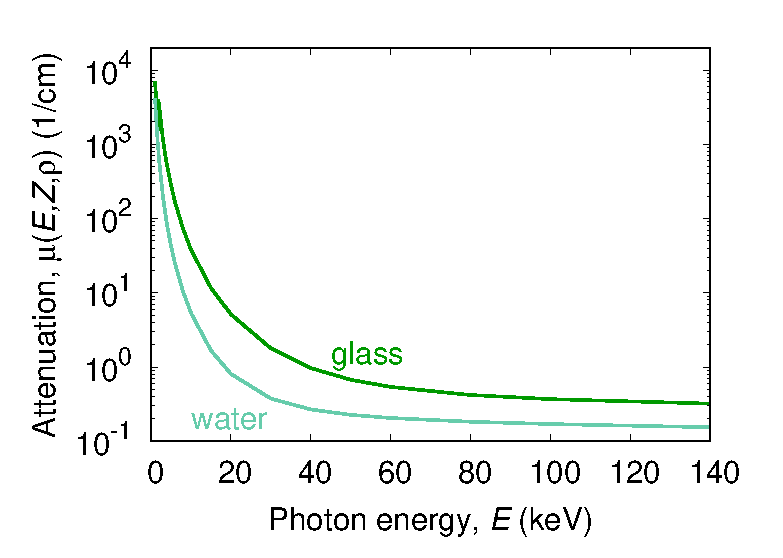
\includegraphics[width=\textwidth]
	{Sources/beam_hardening/Attenuation_vs_energy.eps}}
\end{textblock}
\begin{textblock}{0.48}(0.5,0.9)
	\centering
	\visible<2->{\scriptsize{
		\url{https://www.nist.gov/pml/x-ray-mass-attenuation-coefficients}}}
\end{textblock}

\begin{textblock}{0.45}(0.03,0.14)
	\centering
	\only<1> {%% image of beam through material
	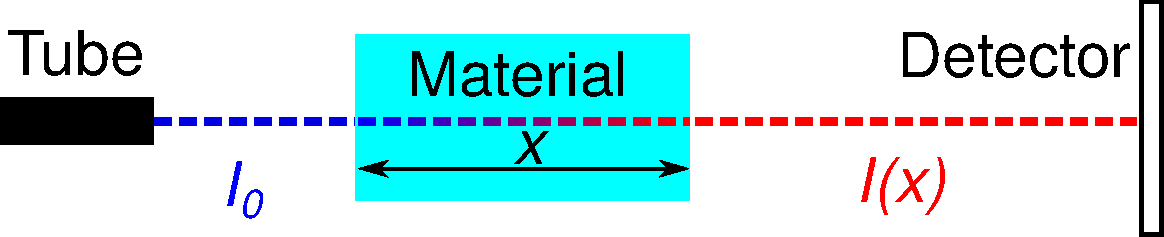
\includegraphics[width=\textwidth]
	{Sources/beam_hardening/beam_through_material.pdf}}
	\only<2>{
	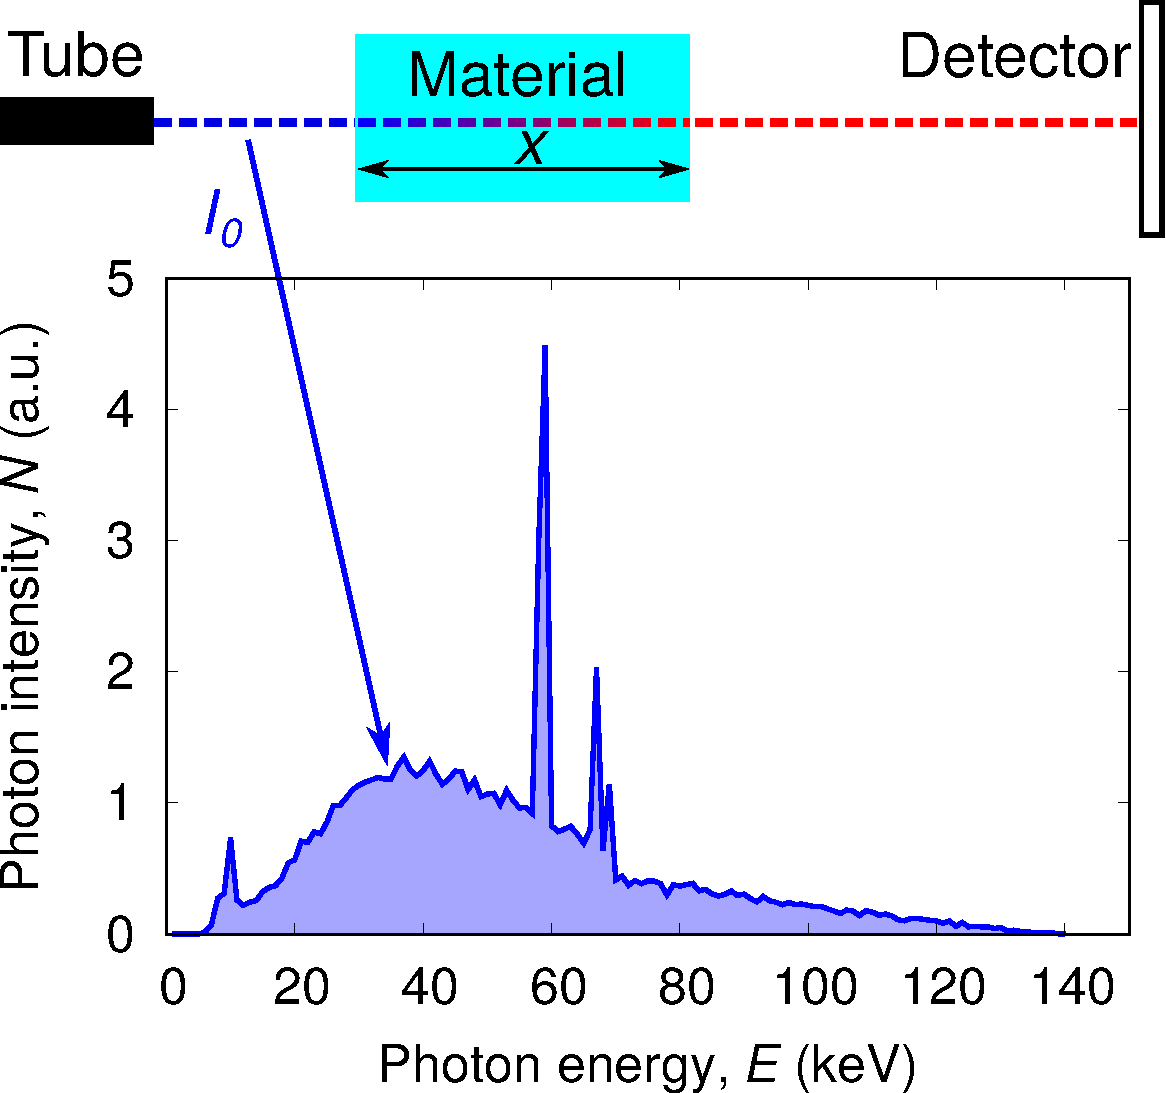
\includegraphics[width=\textwidth]
	{Sources/beam_hardening/x-ray_spectrum_N0.pdf}}
	\only<3>{
	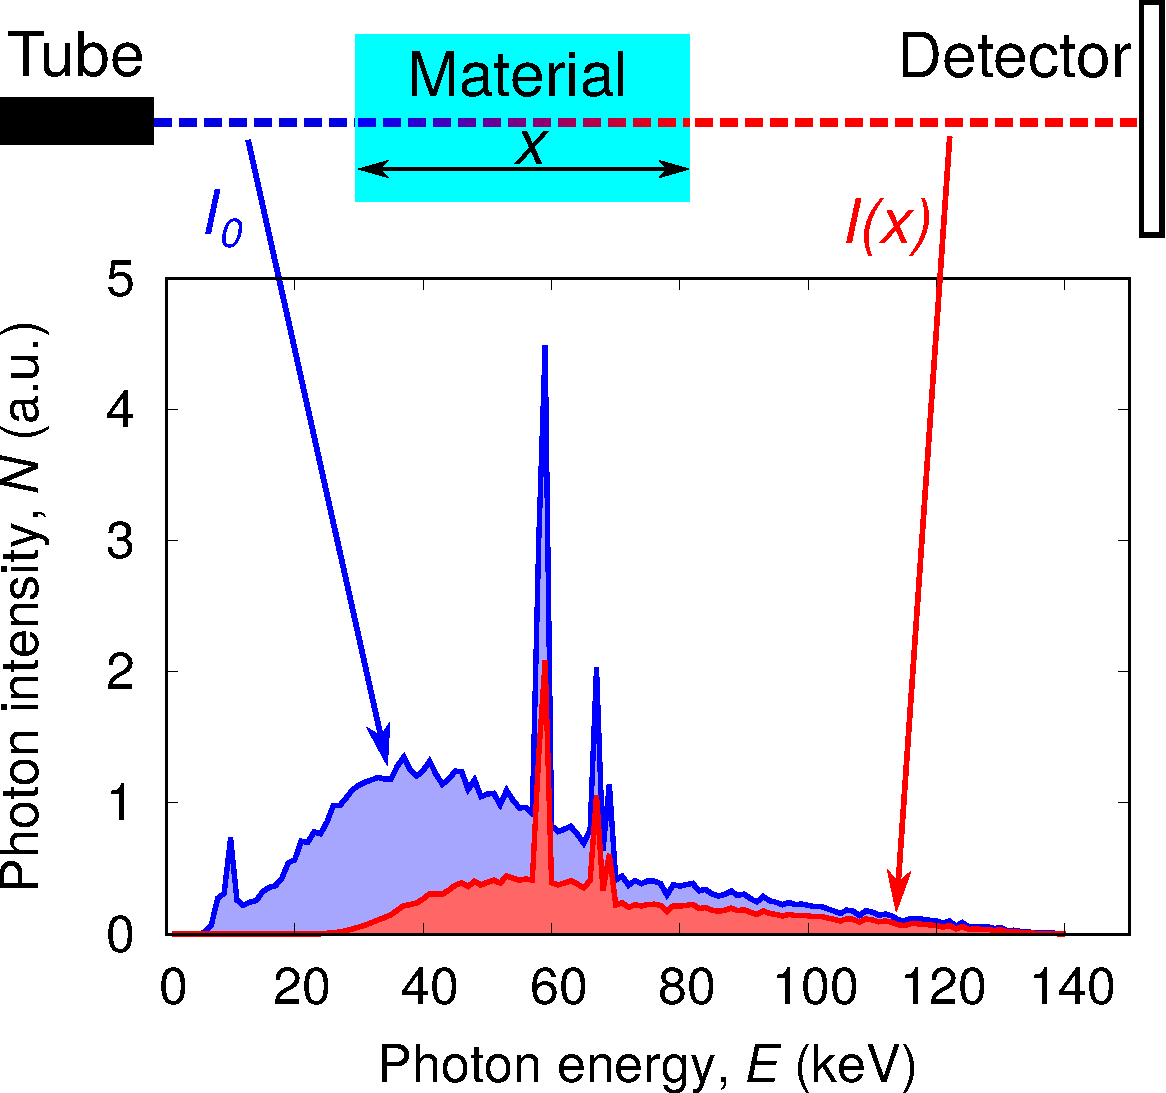
\includegraphics[width=\textwidth]
	{Sources/beam_hardening/x-ray_spectra_beam_hardening.pdf}}
\end{textblock}
\begin{textblock}{0.45}(0.035,0.36)
	\centering
	\only<3>{
	\colorbox{red}{Beam hardening}}
\end{textblock}

}


%%%-------------- The effective attenuation ----------------
\frame{
	\begin{tikzpicture}[remember picture,overlay]
	\fill[blue1]
	(current page.north west) rectangle ([xshift=0.48\textwidth,yshift=0.33\textheight]current page.west|-{pic cs:end});
	\end{tikzpicture}
	
	\begin{textblock}{0.5}(0.02,0.03)
		\textcolor{white}{
			\Large The effective attenuation, $\mu_\text{eff}(x)$}
	\end{textblock}
	
	
	\begin{textblock}{0.45}(0.03,0.1)
		\centering
		\only<1>{
			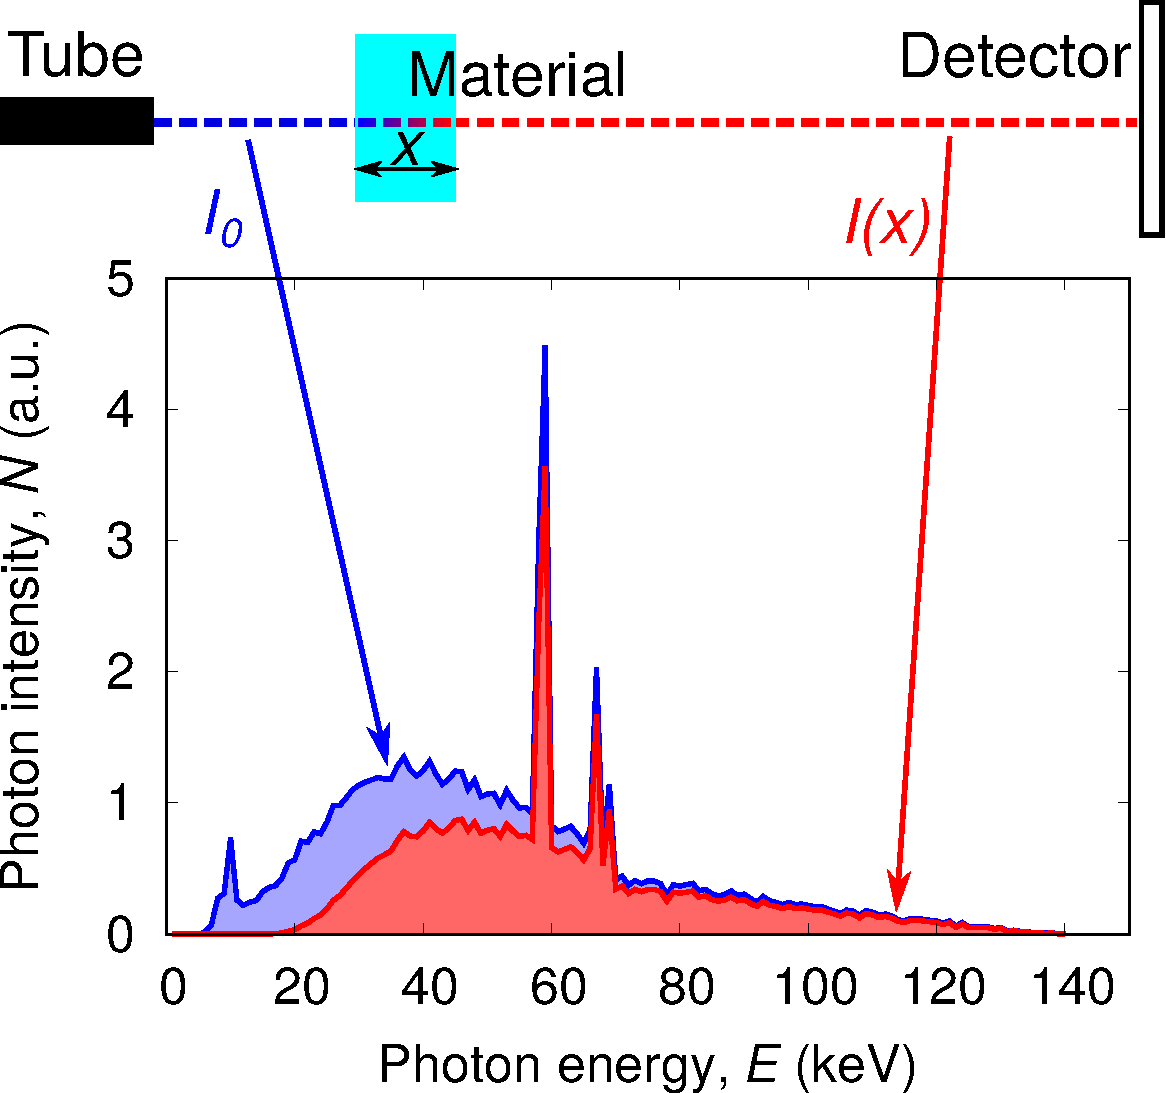
\includegraphics[width=\textwidth]
			{Sources/beam_hardening/x-ray_spectra_beam_hardening_step1.pdf}}
		\only<2>{
			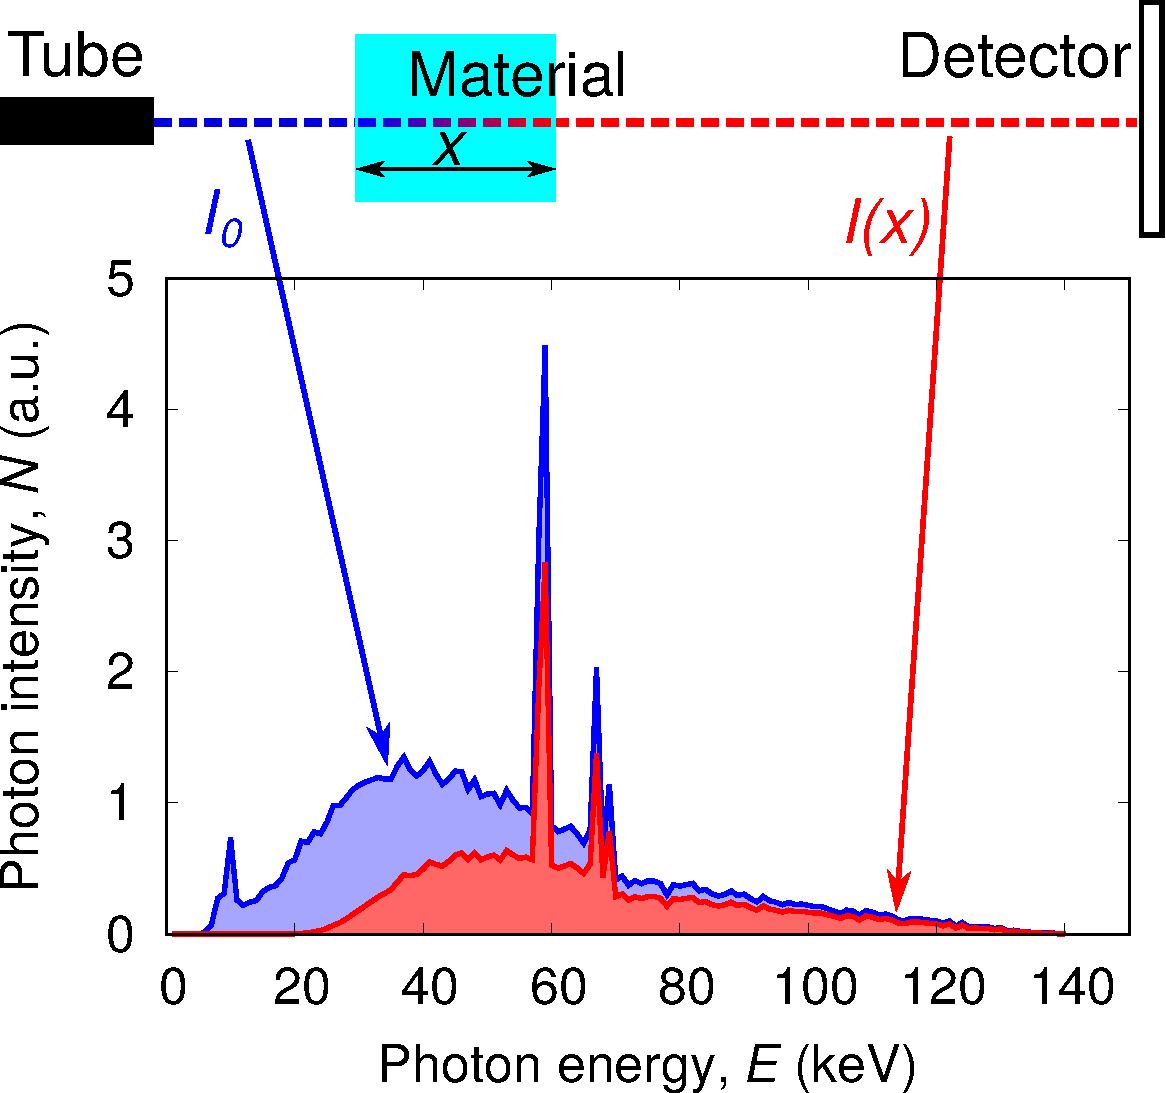
\includegraphics[width=\textwidth]
			{Sources/beam_hardening/x-ray_spectra_beam_hardening_step2.pdf}}
		\only<3,4>{
			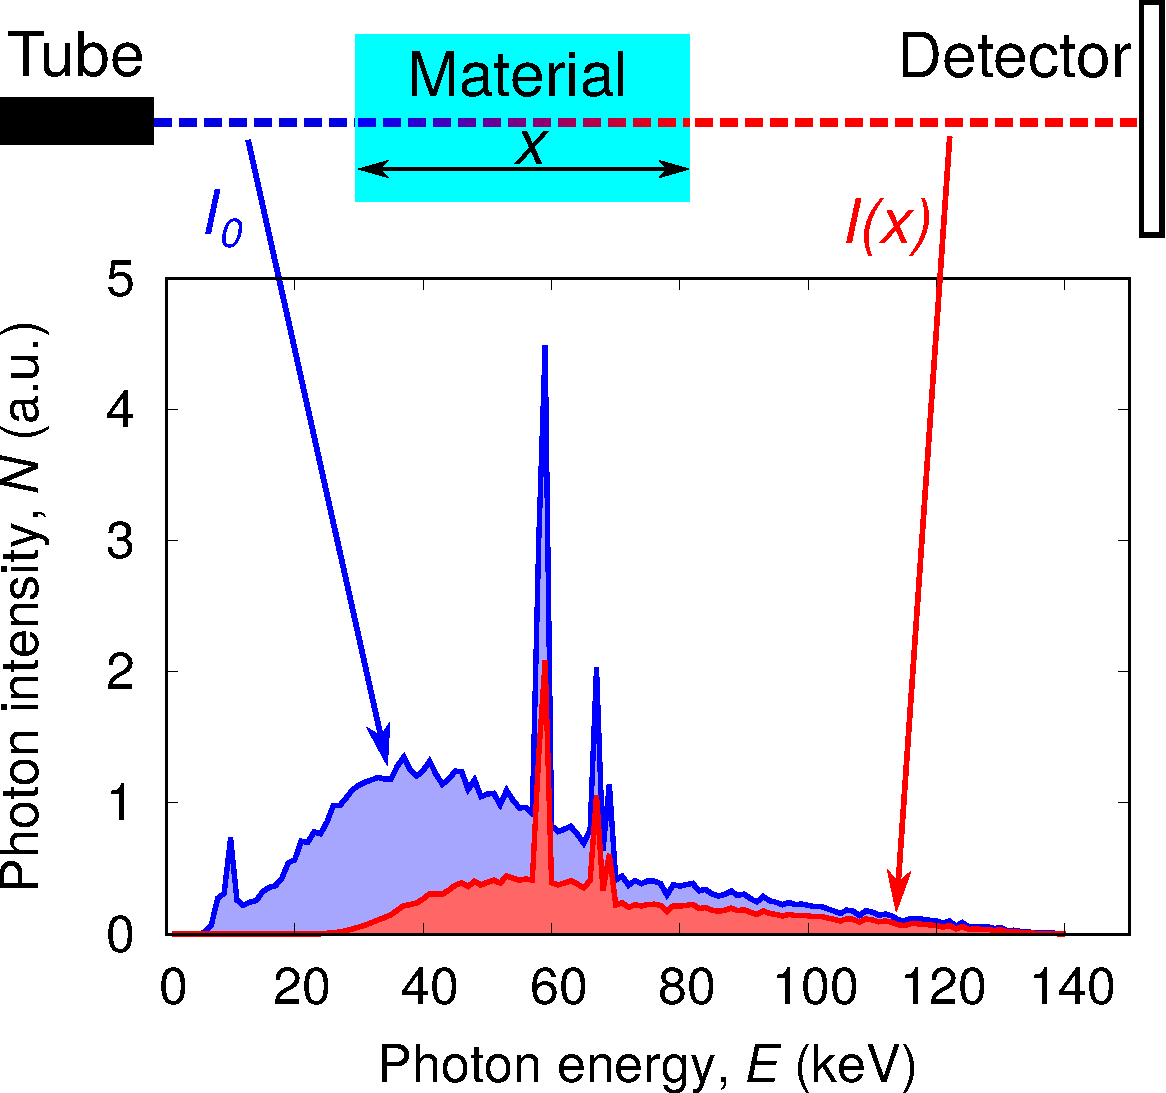
\includegraphics[width=\textwidth]
			{Sources/beam_hardening/x-ray_spectra_beam_hardening.pdf}}
	\end{textblock}
	
	\begin{textblock}{0.17}(0.5,0.02)
		\only<1>{
			\fbox{\parbox{\textwidth}{
					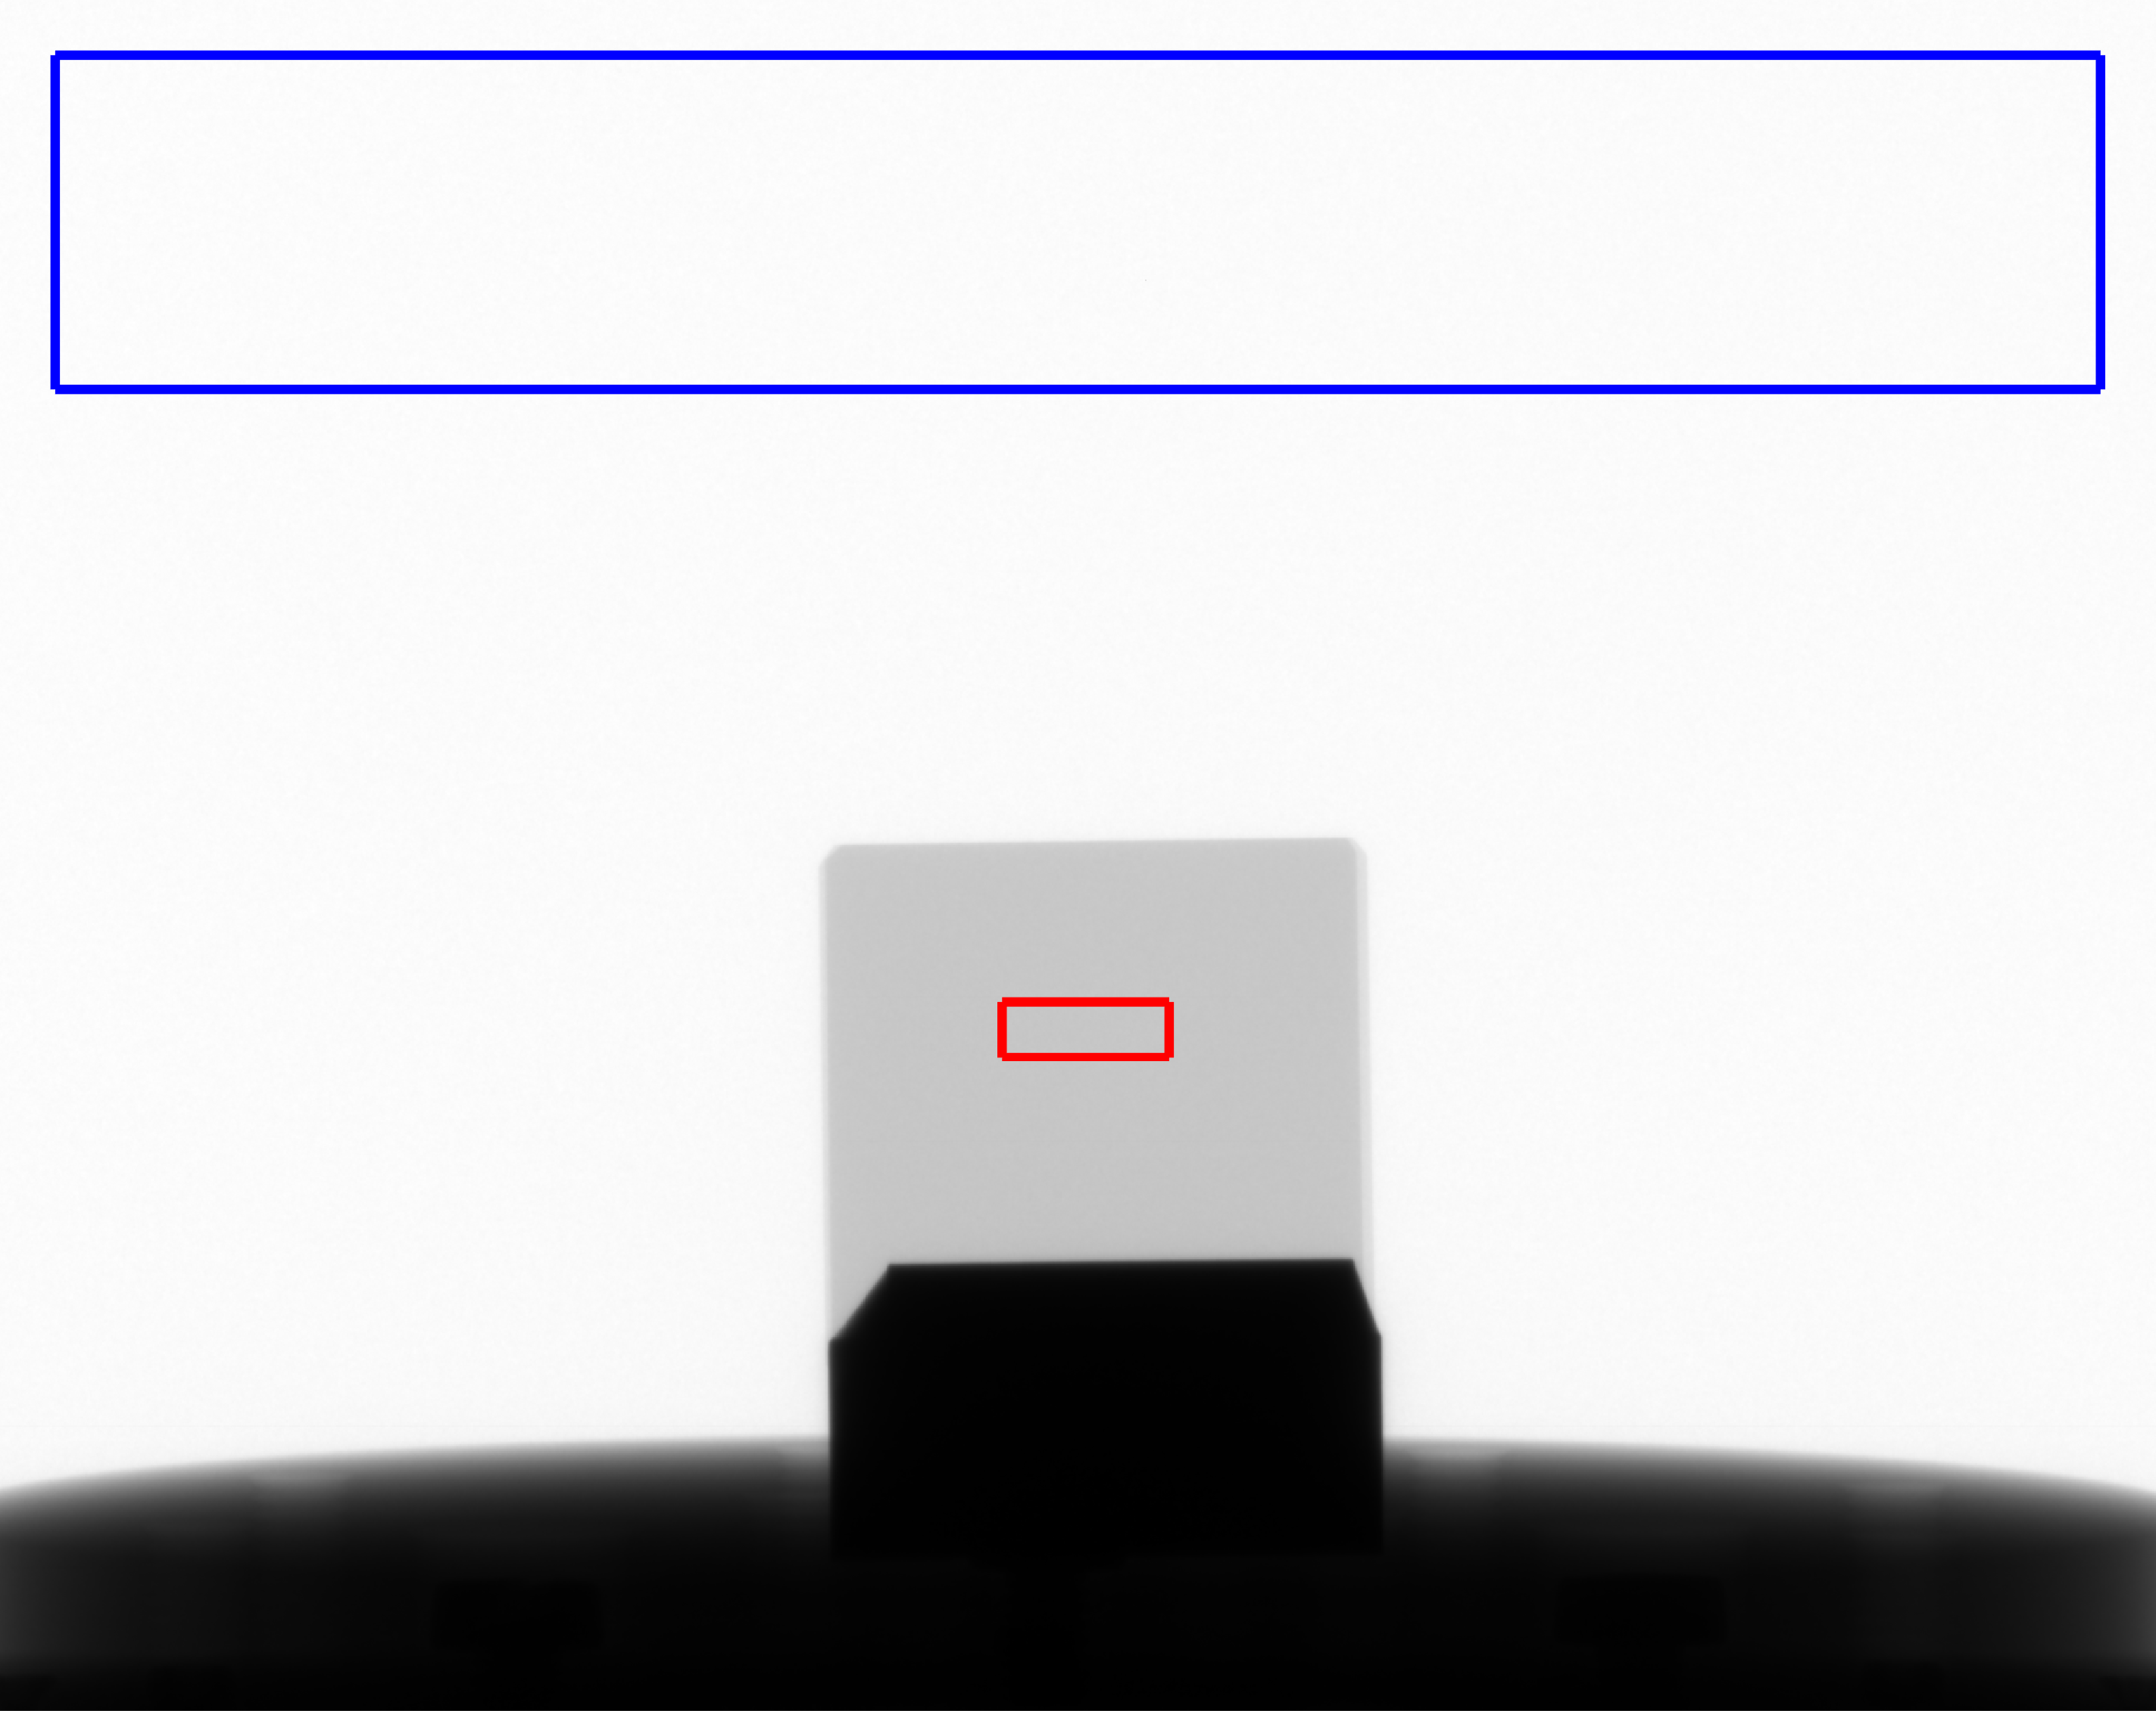
\includegraphics[width=\textwidth]
					{Sources/beam_hardening/02_plates.png}}}}
		\only<2>{
			\fbox{\parbox{\textwidth}{
					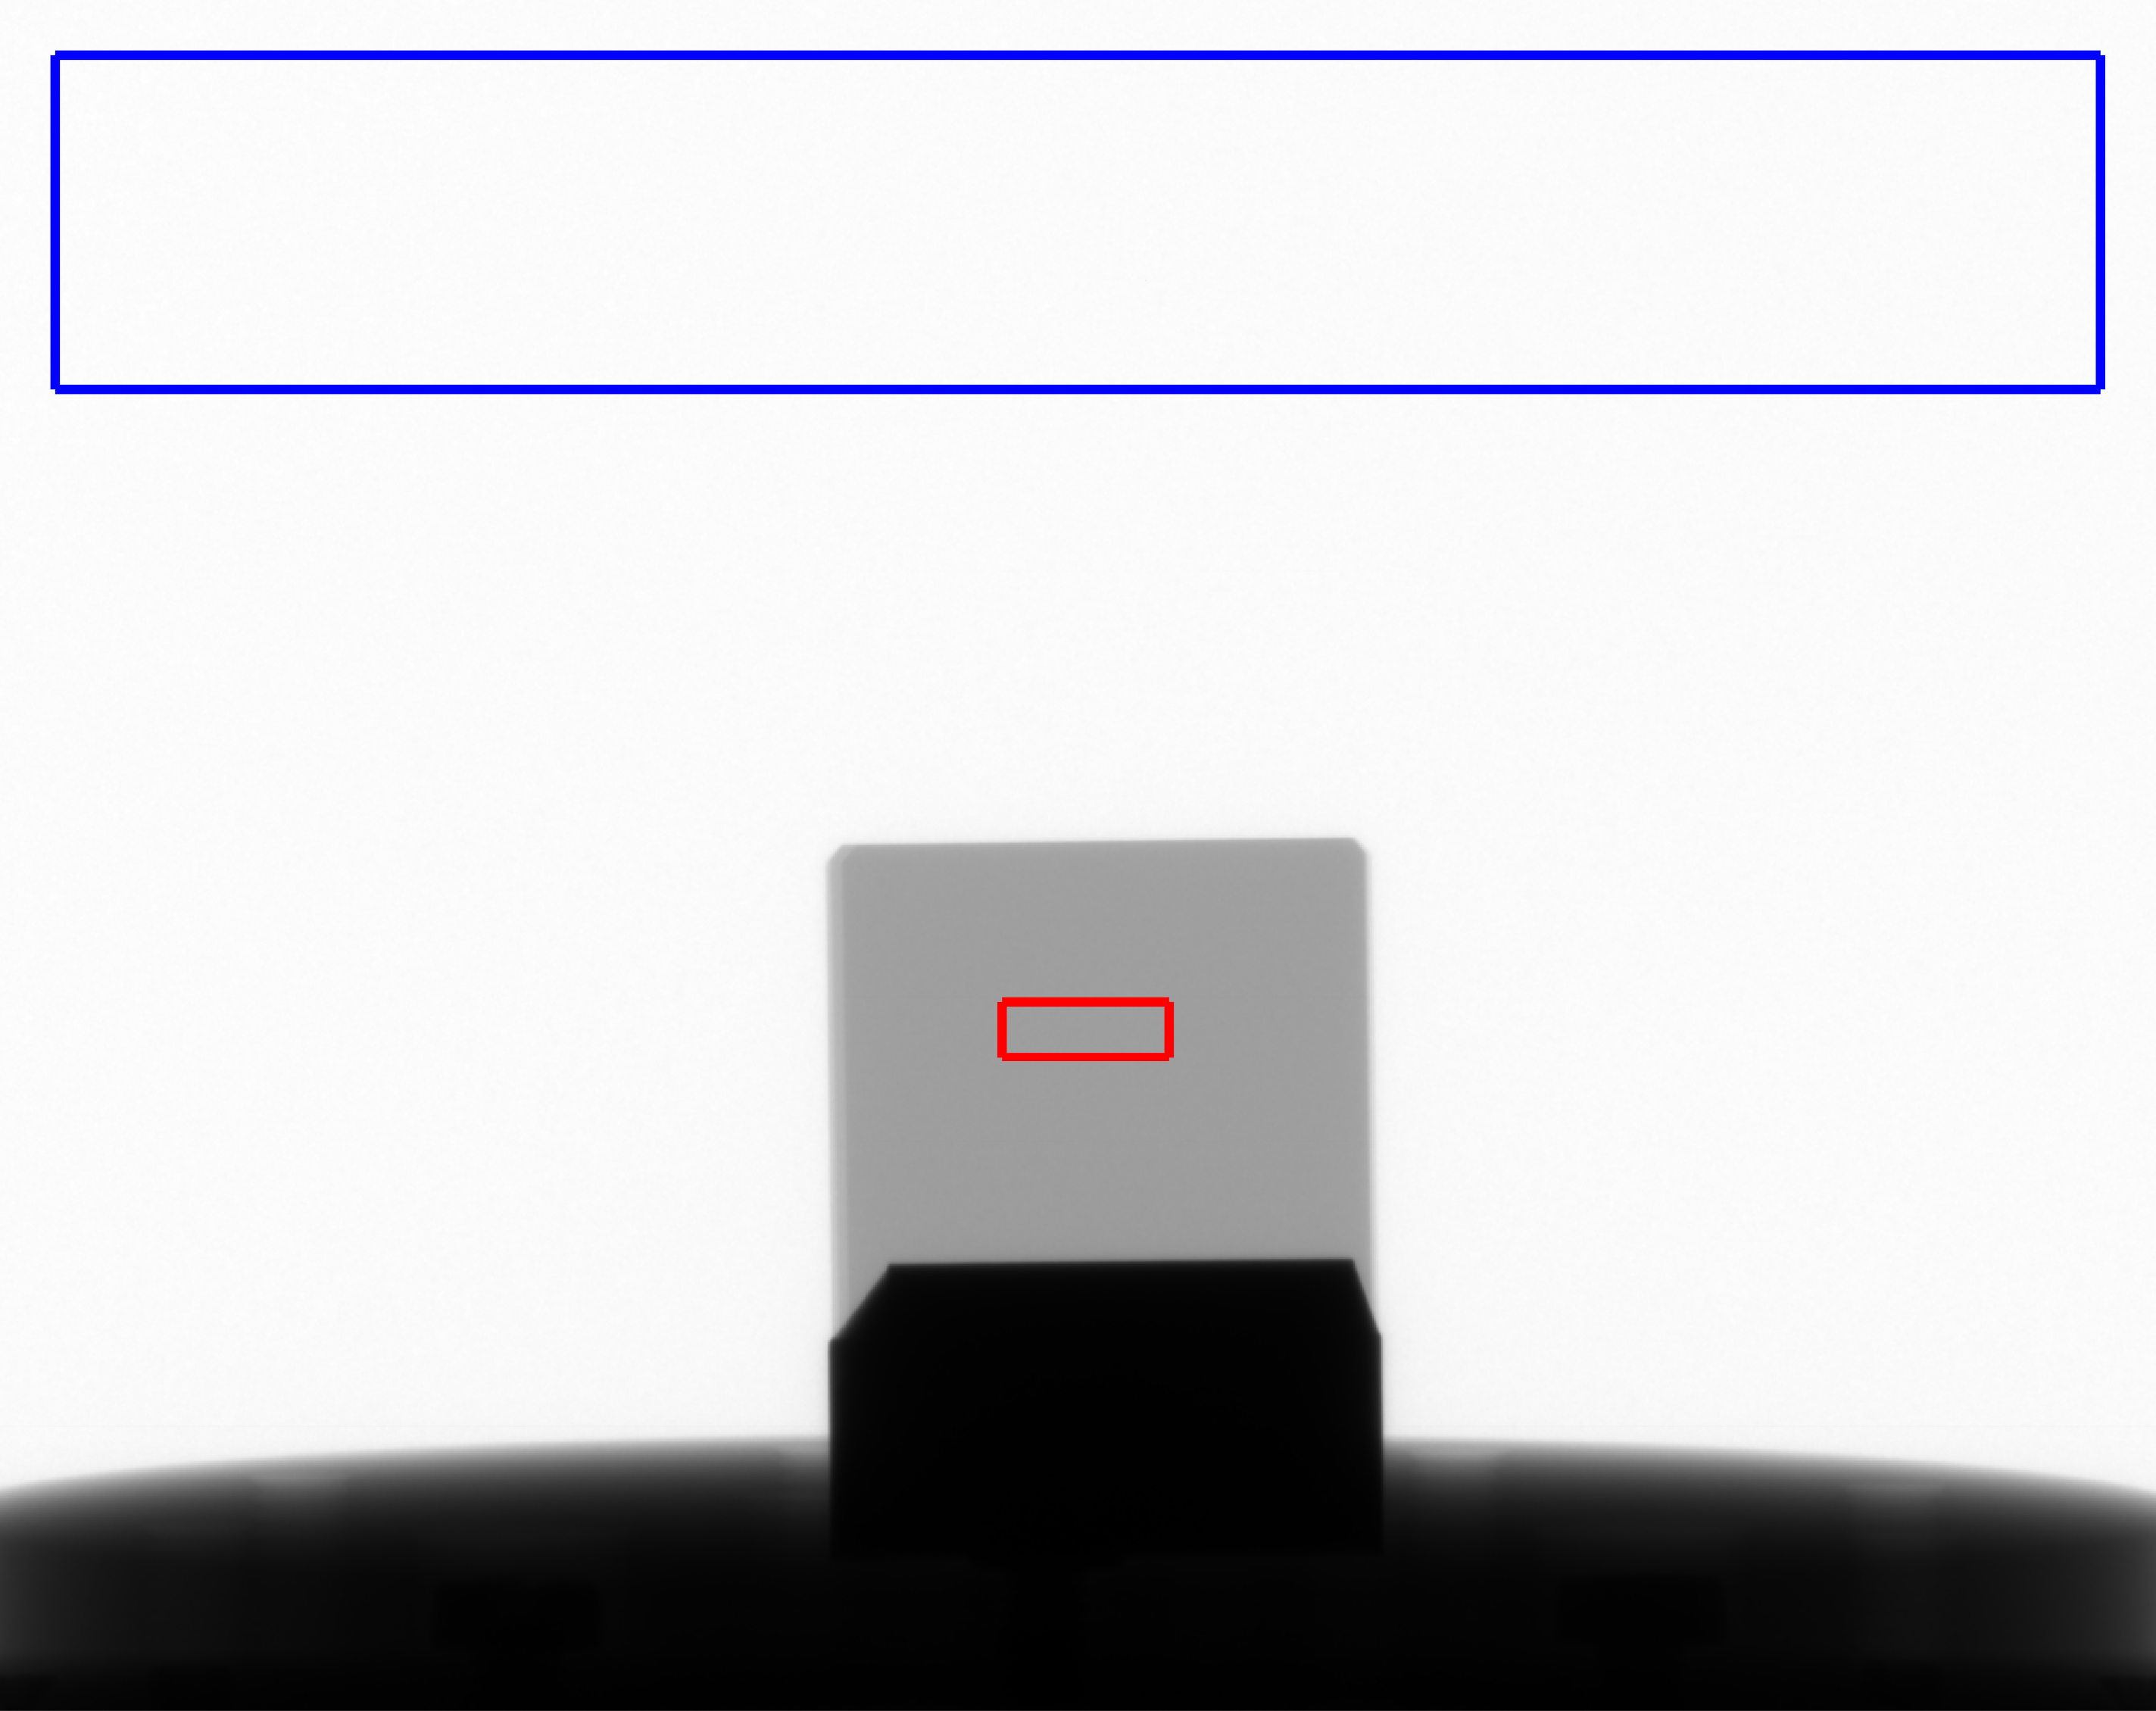
\includegraphics[width=\textwidth]
					{Sources/beam_hardening/04_plates.png}}}}
		\only<3,4>{
			\fbox{\parbox{\textwidth}{
					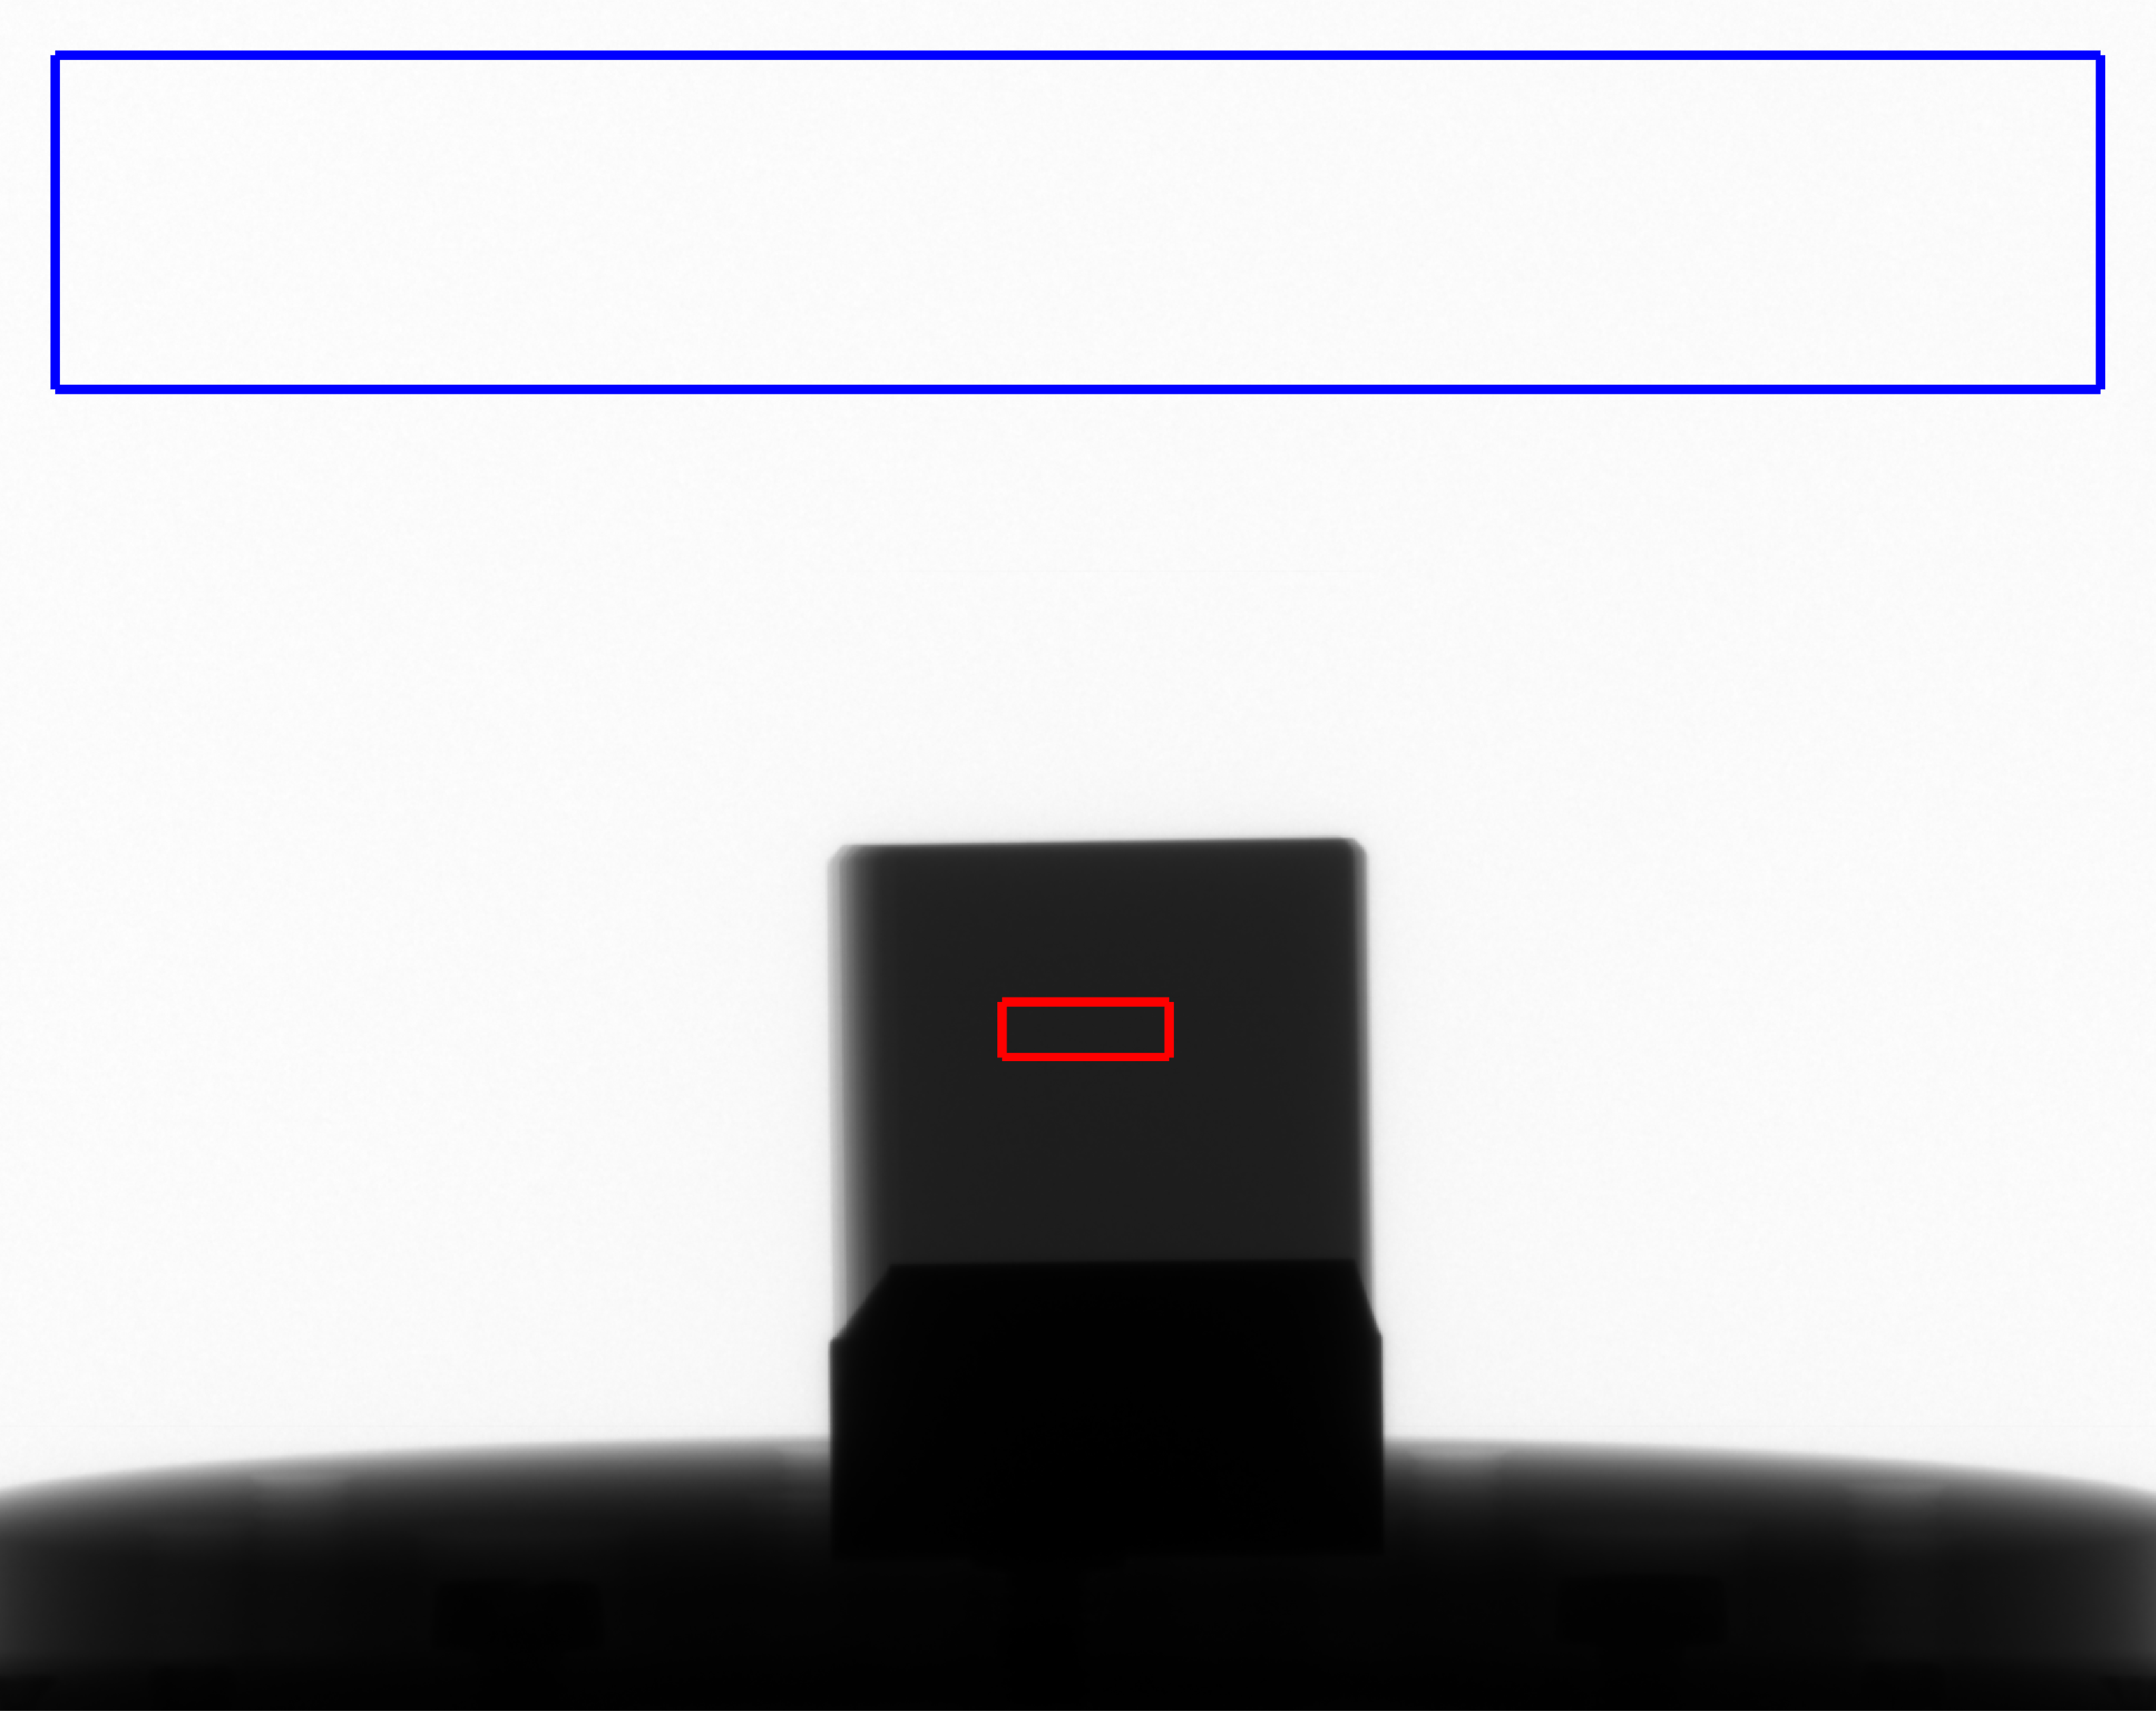
\includegraphics[width=\textwidth]
					{Sources/beam_hardening/20_plates.png}}}}
	\end{textblock}
	
	\begin{textblock}{0.28}(0.7,0.05)
		\only<1,2,3>{
			\textcolor{darkgreen}{\textit{effective}} attenuation:
			\begin{align}
			\textcolor{red}{I(x)} &= 
			\textcolor{blue}{I_0} \exp(- \textcolor{darkgreen}{\mu_\text{eff}(x)}\, x) \nonumber
			\end{align}
		}
		\visible<4->{
			\textcolor{darkgreen}{\textit{effective}} attenuation:
			\begin{align}
			\textcolor{red}{I(x)} &= 
			\textcolor{blue}{I_0} 
			\exp(- \textcolor{darkgreen}{\mu_\text{eff}(x)}\, x) \nonumber\\
			\textcolor{darkgreen}{\mu_\text{eff} (x)} &= - 
			\frac{1}{x} 
			\frac{\textcolor{red}{I(x)}}{\textcolor{blue}{I_0}} \nonumber
			\end{align}
		}
	\end{textblock}
	
	
	\begin{textblock}{0.48}(0.5,0.3)
		\visible<4->{
			\includegraphics[width=\textwidth]
			{Sources/beam_hardening/attenuation_boro_glass_140kV.pdf}}
	\end{textblock}
	
	\begin{textblock}{0.15}(0.8,0.4)
		\centering
		\visible<4->{
			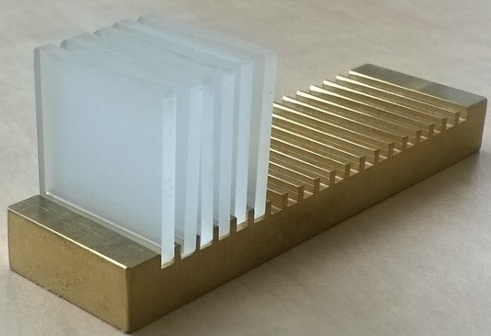
\includegraphics[width=\textwidth]
			{Sources/beam_hardening/plates_on_slide.png}}
	\end{textblock}
	
	
}
